\chapter{Introduction}\label{introduction}

The Roa Logic AHB-Lite Memory IP is a fully parameterized soft IP
implementing on-chip memory for access by an AHB-Lite based Master. 
All signals defined in the \emph{AMBA 3 AHB-Lite v1.0} specifications are
fully supported.

The IP supports a single AHB-Lite based host connection and enables
address \& data widths, memory depth \& target technology to be
specified via parameters. An option to register the memory output is
also provided.

\begin{figure}[th]
	\centering
	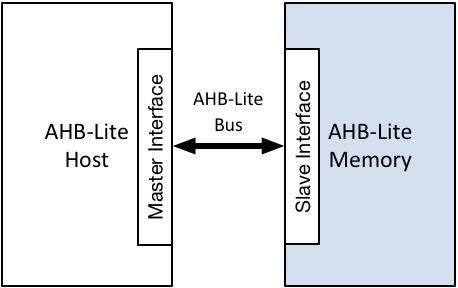
\includegraphics{img/AHB-Lite-Memory-SysDiag.png}
	\caption{AHB-Lite Memory System}
	\label{fig:ahb-lite-memory-sysdiag}
\end{figure}

\section{Features}\label{features}

\begin{itemize}
\item
  Full support for AMBA 3 AHB-Lite protocol
\item
  Fully parameterized
\item
  User-defined address and byte-aligned data widths supported
\item
  Configurable memory depth, limited only by target technology
  capability
\item
  Technology-specific memory cells instantiated automatically
\item
  Combinatorial or registered data output
\end{itemize}